\pattern{Composite}
\begin{summary}
Used to manage a hierarchy of components, each of which could be a composite,
or a leaf. Components use a single interface, which allows the user to call
methods without having to know which type of component it is. Every component
can be treated as its own entity thus allowing the whole system to be broken
down into parts.  

The main theme of the {\bf Composite} pattern is ``Containers that contain elements,
each of which could also be a container''

The composite design pattern should be applied when multiple objects are being
used in the same way in which each object has nearly identical code.
Additionally if the client does not care about the type of object it interacts
with than the composite design pattern is a good choice as it allows the client
to operate on objects without the concern for type.
\end{summary}

\subsubsection{Vocabulary}
\begin{description}[noitemsep]
\item[Client] Only aware of Leafs/Composites through the Component Interface
\item[Component] An item in the composite pattern, that can either be a leaf or a composite
\item[Leaf] Primitive component that cannot contain other components
\item[Composite] Component than can contain other components
\item[Topology] The composite pattern is most often used to represent
hierarchies and tree structures. Composites contained in another composite
represent a subsystem and are functional without knowledge of its parent.
\end{description}


\comparison{\begin{itemize}
\item Readability: The composite pattern simplifies client code that interacts
with complex tree structures, since the user does not have to know if they are
dealing with a leaf or a composite.
\item Evolvability: Makes it easier to add new kinds of components. New
components will work with existing client code without client needing to
change.
\end{itemize}

}{\begin{itemize}
\item Adaptability: all classes in the hierarchy follow a similar interface,
    which can lead to an overly general design. Therefore it is more difficult
    to restrict the components of a composite. Since all the classes implement
    an abstract interface this is not possible without a run-time check for the
    desired components.
\item Evolvability: the composite pattern will increase change resilience
    for adding specific properties or restrictions to components, since
    different types of components are often treated uniformly.
\end{itemize}
} %END comparison

\begin{nfps}
\item[Adaptability] The composite design pattern forces containers to work with
    child nodes through a common interface which allows for recursive
    operations on the entire hierarchy. This means that as new compositions and
    leaves are added to the hierarchy they can adapt to the existing code.
\item[Low Complexity] All classes follow a similar interface so the client
    does not have to worry about class specific code. The client can just treat
    primitives and composites as homogenous classes.
\item[Low Coupling] The composite design pattern reduces coupling by utilizing
    the same interface for each of the components. Whether it is a leaf or a
    composite, the class does not need to know any information about the other
    classes. 
\end{nfps}

\subsubsection{Example}
Using the composite pattern in this example lets the user interact with the
entire hierarchy easily, lets them break the tree into subtrees, and allows
users to add new type of components if it is necessary in the future.
Note that {\sc Folder} implements {\sc add()} and {\sc remove()} which are not
declared in the interface. There are cases where both types of components must
have the exact same interface, thus occasionally these functions are declared
in the component, but would cause an error if the user tries to add to a leaf.

\begin{center}
    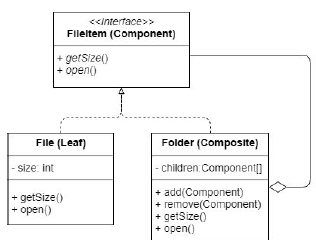
\includegraphics[width=0.4\textwidth]{./composite1}
    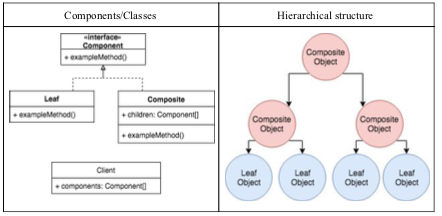
\includegraphics[width=0.5\textwidth]{./composite2}
\end{center}
